\subsection{Design and architecture of ITU-MiniTwit}

The architecture is depicted through UML diagrams conforming to the 3+1 architecture model~\cite{drawio}. These are Module, Component-and-Connector and Allocation Views. Moreover, a Container Diagram is supplied to utilize the methodology of the C4model~\cite{c4model}. All graphs are contained in .xml files on the GitHub repository and can be reimported to the website to make future changes~\cite{architecturalViews}. The following list enumerates services embedded within the project, therefore included in the diagrams:

\begin{itemize}[noitemsep]
    \item MiniTwit Vue.js Web Application
    \item MiniTwit .NET Application
    \item Prometheus
    \item Grafana
    \item DataDog Agent
    \item Database: MariaDB
\end{itemize}

\vspace{3mm}

Interactions among those is achieved with the support of the following technologies, frameworks, cloud providers and services:

\begin{itemize}[noitemsep]
    \item DigitalOcean
    \item Docker
    \item TravisCI
    \item SonarQube
    \item Snyk - Docker Scan
    \item DataDog web server
    \item Grafana Dashboard
\end{itemize}

\subsubsection*{Module View}

This section provides us with three levels of abstractions of important set of functionalities that make up the system.
\vspace{3mm}

\underline{1. High Level Module View}
\vspace{3mm}

The view provides us with the high-level functionality of the project. Connections by arrows display dependent relationships between abstract packages.

\begin{figure}[h!]
    \centering
    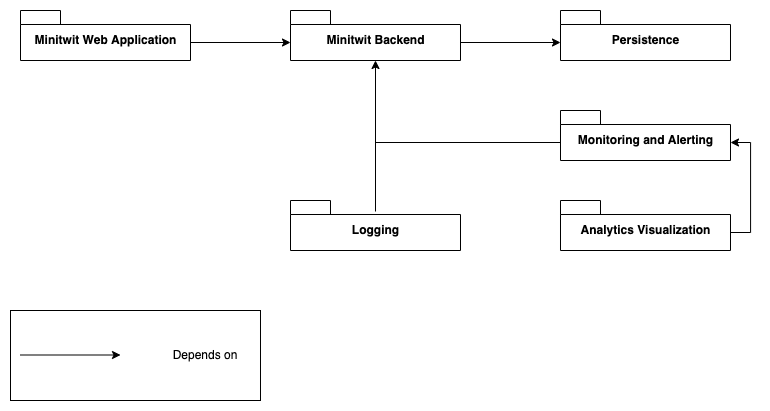
\includegraphics[width=\linewidth,height=\textheight,keepaspectratio]{images/architectural_views/minitwit_module_view_high_level.png}
    \caption{High level module view~\cite{moduleViewHighLevel}.}
    \label{fig:moduleview}
\end{figure}

\newpage

\underline{2. Layers of backend application}
\vspace{3mm}

This zoomed-in view with the architecture of the backend application shows the layering consisting of the Api, Domain Service and Persistence Layer.

\begin{figure}[h!]
    \centering
    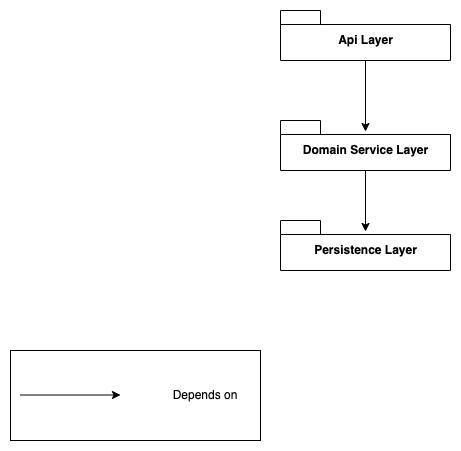
\includegraphics[width=0.5\textwidth]{images/architectural_views/minitwit_module_view_backend_layers.png}
    \caption{Layers of back-end~\cite{moduleViewLayers}.}
    \label{fig:modulebackend}
\end{figure}

\newpage
\underline{3. Layers detailed}
\vspace{3mm}

Focusing more into the architecture of the backend reveals a more in-depth structure of the layers. Controllers are dependent on DomainService classes that has access to Models representing data incoming from the Persistence Layer.

\begin{figure}[h!]
    \centering
    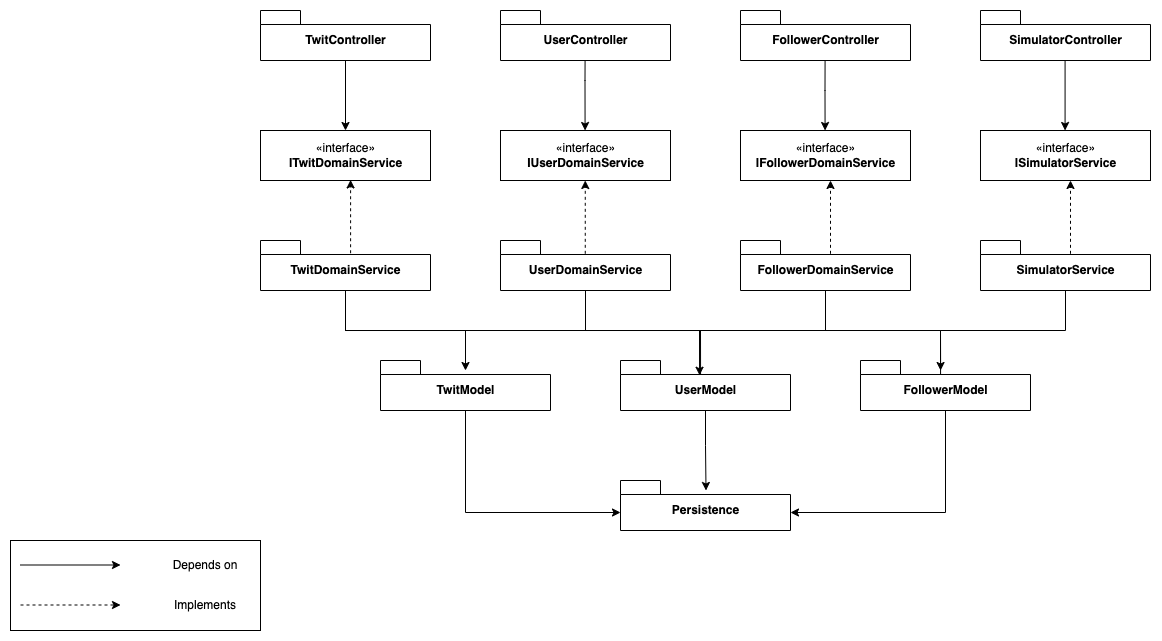
\includegraphics[width=\linewidth,height=\textheight,keepaspectratio]{images/architectural_views/minitwit_module_view_backend_layers_detailed.png}
    \caption{Layers detailed~\cite{moduleViewLayersDetailed}.}
    \label{fig:modulebackenddetail}
\end{figure}

\newpage
\subsubsection*{Component-and-Connector View}

The view displays high-level communication between the subsystems and how they should work as a whole. Connections are defined by various communication channels and their protocols.
\vspace{3mm}

Apart from the usual interaction of the browser, web and back-end application trio, the Docker Swarm component introduces few key interactions. The back-end application plays a key role as it queries resources from the database, while providing metrics via Serilog and DataDog Agent to the DataDog Logging Service. It also communicates with SonarQube - the Static Code Analysis tool in the form of analysis reports.System telemetries are gathered and envisioned with the interaction of Prometheus and Grafana. The metrics pulled from the back-end application by Prometheus are gathered by Grafana using PromQL. It is then displayed on dashboards to analyse those.
\vspace{3mm}

\begin{figure}[h!]
    \centering
    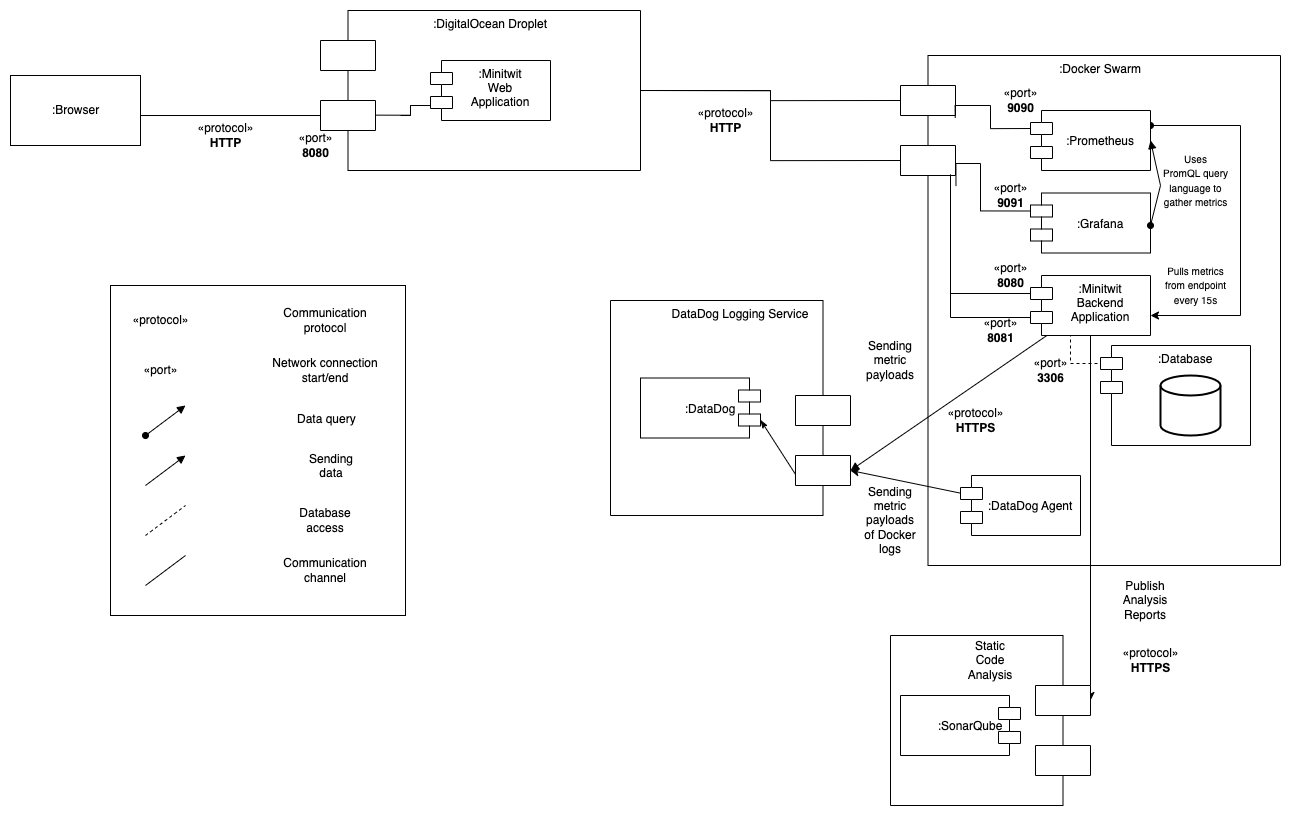
\includegraphics[width=\linewidth,height=\textheight,keepaspectratio]{images/architectural_views/minitwit_cc_view.png}
    \caption{Component-and-Connector View ~\cite{componentAndConnectorView}}
    \label{fig:ccview}
\end{figure}

\subsubsection*{Allocation View}

The extensive graph can be seen on \ref{fig:allocationview}. This view maps different parts of the system to their respective deployment environments. Information about cloud providers, module arrangement into a cluster, device properties and executables contained in execution environments can be extracted from this perspective.

\begin{sidewaysfigure}
    \centering
    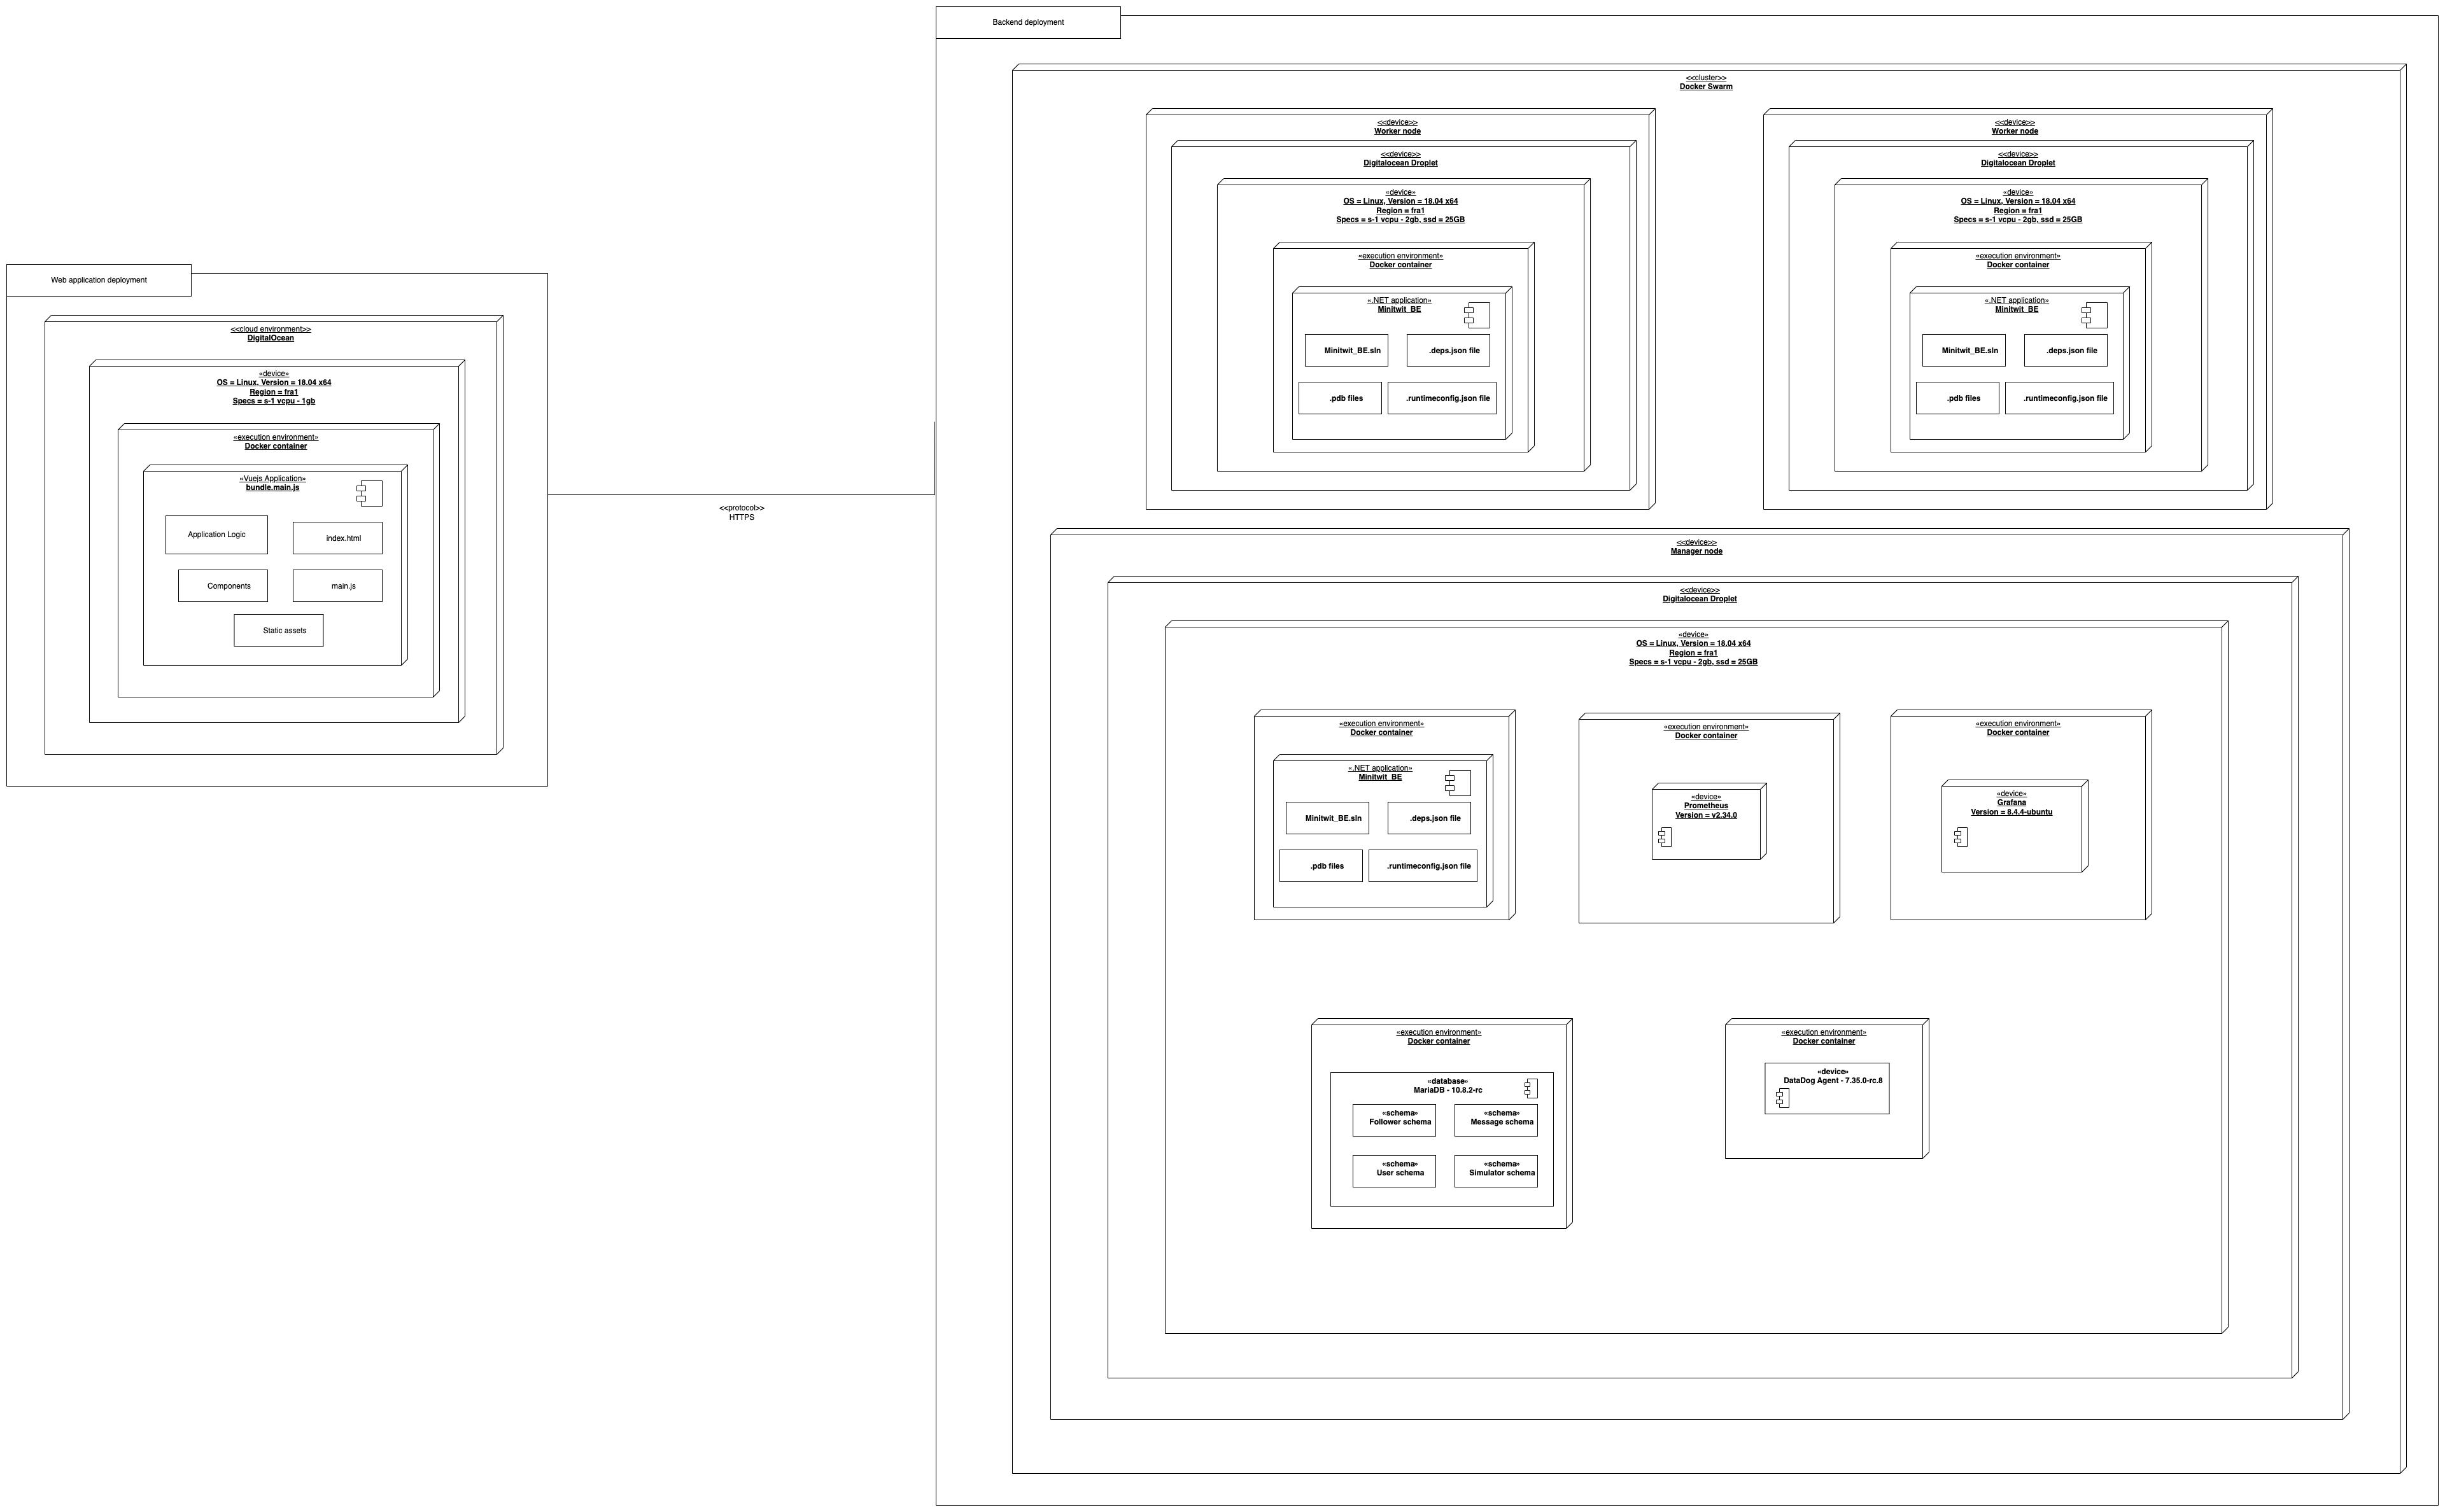
\includegraphics[scale=0.18]{images/architectural_views/minitwit_allocation_view.png}
    \caption{Allocation view ~\cite{allocationView}}
    \label{fig:allocationview}
\end{sidewaysfigure}



\newpage
\subsubsection*{Container Diagram}

The Container Diagram details how changes of these subsystems get deployed into production. Flow of change can be followed from submitted local modifications checked into the appropriate branches triggering the continuous integration and delivery pipeline’s different stages, to the deployment into production on cloud environments.

\begin{figure}[h!]
    \centering
    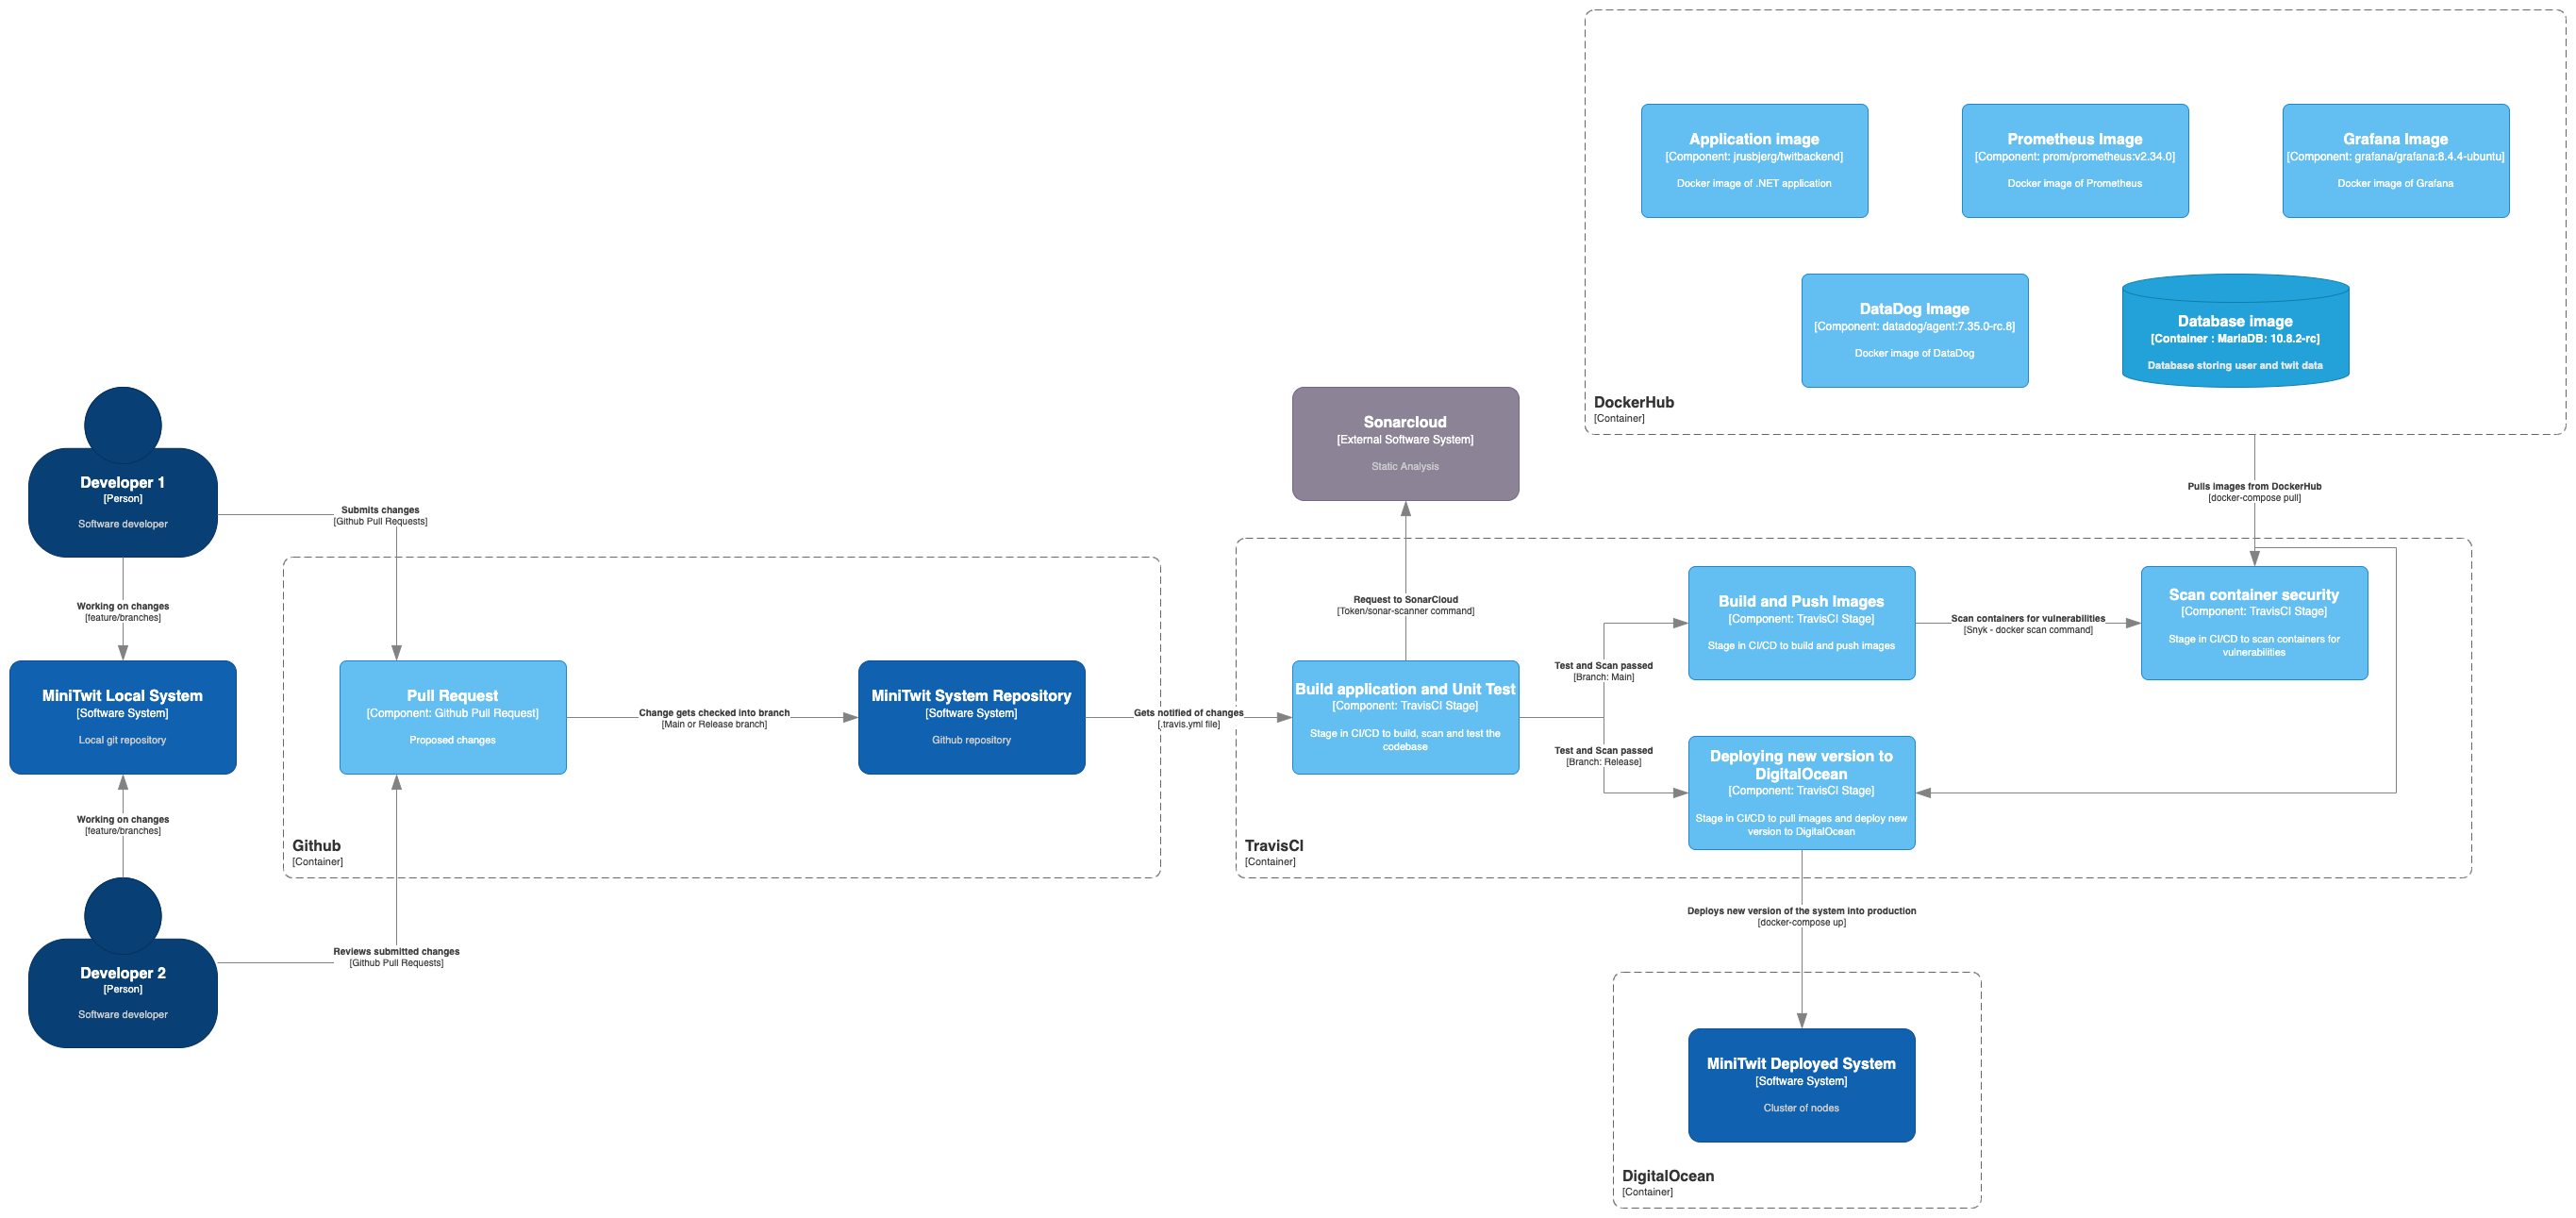
\includegraphics[width=\linewidth,height=\textheight,keepaspectratio]{images/architectural_views/workflow_of_change.png}
    \caption{Container Diagram ~\cite{containerDiagram}}
    \label{fig:containerdiagram}
\end{figure}